\documentclass[german,  % Standardmäßig deutsche Eigenarten, englisch -> english
parskip=full,  % Absätze durch Leerzeile trennen
%bibliography=totoc,  % Literatur im Inhaltsverzeichnis (ist unüblich)
%draft,  % TODO: Entwurfsmodus -> entfernen für endgültige Version
headsepline]{scrartcl}
\usepackage[utf8]{inputenc}  % Kodierung der Datei
\usepackage[T1]{fontenc}  % Vollen Umfang der Schriftzeichen
\usepackage[german]{babel}  % Sprache auf Deutsch (neue Rechtschreibung)
\usepackage{booktabs}
\usepackage{float}
% Mathematik und Größen
\usepackage{amsmath}
\usepackage[locale=DE,  % englische Eigenarten, deutsch -> DE
separate-uncertainty,  % Unsicherheiten seperat angeben (mit ±)
]{siunitx}
%http://texdoc.net/texmf-dist/doc/latex/siunitx/siunitx.pdf
\usepackage{physics}  % Erstellung von Gleichungen vereinfachen
\usepackage{svg}    
\usepackage{graphicx}  % Bilder einbinden \includegraphics{Pfad/zur/Datei(ohne Dateiendung)}
\usepackage[
backend=biber,
style=nature,
sorting=ynt
]{biblatex}
\usepackage{wrapfig}
\usepackage[version=4,arrows=pgf]{mhchem}  % Chemie Paket für Isotopenschreibweise etc.
\usepackage{wrapfig}
\usepackage{floatflt}
\usepackage{enumerate}
\usepackage{url}
% Gestaltung
%\usepackage{microtype}  % Mikrotypographie (kann man am Ende verwenden)
\usepackage{booktabs}  % schönere Tabellen
%\usepackage[toc]{multitoc}  % mehrspaltiges Inhaltsverzeichnis
\usepackage{multicol}
\usepackage{csquotes}  % Anführungszeichen mit \enquote
\usepackage{caption}  % Anpassung der Bildunterschriften, Tabellenüberschriften
\usepackage{subcaption}  % Unterabbildungen, Untertabellen, …
\usepackage{cprotect}
\usepackage{enumitem}  % Listen anpassen
\usepackage{siunitx}
\usepackage{eufrak}
\usepackage{dirtytalk}
\usepackage{subcaption}
\usepackage{textcomp}
\setlist{itemsep=-10pt}  % Abstände zwischen Listenpunkten verringern
\addbibresource{bib_su2.bib}
% Manipulation des Seitenstils
\usepackage{scrlayer-scrpage}
% Kopf-/Fußzeilen setzen
\pagestyle{scrheadings}  % Stil für die Seite setzen
\clearscrheadings  % Stil zurücksetzen, um ihn neu zu definieren
\automark{section}  % Abschnittsnamen als Seitenbeschriftung verwenden
\ofoot{\pagemark}  % Seitenzahl außen in Fußzeile
\ihead{\headmark}  % Seitenbeschriftung mittig in Kopfzeile
%\setkomafont{\headsepline}{}
\setcounter{tocdepth}{2} %set depth of printed table of contets.

\makeatletter

%\renewcommand\tableofcontents{% Absatz vor Gliederungspunkten
   % \begin{multicols}{2}[\section*{\contentsname
 %       \@mkboth{%
  %         \MakeUppercase\contentsname}{\MakeUppercase\contentsname}}]%
 %   \@starttoc{toc}%
 %   \end{multicols}%
 %   }

\makeatother %print dots in sections in toc.

\usepackage[hidelinks]{hyperref}  % Links und weitere PDF-Features
\usepackage{hyperref}
\hypersetup{
    colorlinks=true,
    linkcolor=blue,
    citecolor=red,
    filecolor=magenta,      
    urlcolor=cyan,
    pdftitle={Overleaf Example},
    pdfpagemode=FullScreen,
    }
\usepackage[]{cleveref} %noabbrev für ausgeschriebene verweise
% TODO: Titel und Autor, … festlegen
\newcommand*{\titel}{Supraleitung II}
\newcommand*{\autor}{Lukas König, Steven Gebel}
\newcommand*{\abk}{}
\newcommand*{\betreuer}{Dr. Sergey Granovsky}
\newcommand*{\messung}{5. November 2021}
\newcommand*{\ort}{REC/D106}
\newcommand{\diff}[1]{\frac{\mathrm{d}}{\mathrm{d}#1}}
\newcommand{\mum}{\:\si{\mu m\:}}
\newcommand{\ten}[1]{\cdot10^{#1}}
\newcommand{\dsys}{\Delta_\text{sys}}
\newcommand{\logdiff}[1]{\left(\frac{\Delta #1}{#1}\right)^2}
\newcommand{\dunderline}[1]{\underline{\underline{#1}}}
\newcommand{\bcref}[1]{\namecref{#1} \textcolor{blue}{\labelcref{#1}}}

\hypersetup{pdfauthor={\autor}, pdftitle={\titel}}  % PDF-Metadaten setzen

% automatischen Titel konfigurieren
\titlehead{Fortgeschrittenenpraktikum SU II\abk \hfill Technische Universität Dresden}
\subject{Praktikumsbericht}
\title{\titel}
\author{\autor}
\date{\begin{tabular}{ll}
Protokoll: & \today\\
Messung: & \messung\\
Ort: & \ort\\
Betreuer: & \betreuer\end{tabular}}
\begin{document}
\begin{titlepage}
\maketitle  % Titel setzen
\tableofcontents  % Inhaltsverzeichnis setzen
\end{titlepage}
\section{Einleitung}
\subsection{Aufgabenstellung}
    \begin{enumerate}
        \item Einkühlen eines LHe-Badkryostaten
        \item Bestimmung des kritischen Magnetfelds $H_c$ für eine Blei-Probe als Funktion der Temperatur im Temperaturbereich $1.5 \si{K}$ und $10 \si{K}$
        \item Konstruktion der Phasenlinie zwischen supraleitendem und normaleitendem Zustand und Vergleich mit Vorhersagen der BCS-Theorie und Literaturwerten
    \end{enumerate}

\subsection{Theoretischer Hintergrund}
Die Supraleitung findet in der heutigen Forschung sehr viele Anwendungen um besonders starke Magnetfelder zu erzeugen (z.B. im Large Hadron Collider LHC am CERN).\\
Grund dafür ist, dass Materialien, die in den supraleitenden Zustand wechseln können, in diesem keinen elektrischen Widerstand mehr besitzen und ideale Diamagneten sind.\\
In diesem Versuch werden die Eigenschaften eines Supraleiters 1. Art untersucht. \\
\\Supraleiter 1. Art bestehen oft aus metallischen Elementen und besitzen meistens sehr niedrige kritische Temperaturen $T_c$. Unterhalb dieser kritischen Temperaturen findet der Übergang in den supraleitenden Zustand statt.\\
Dieser supraleitende Zustand kann zerstört werden, wenn die Temperatur erhöht wird $T > T_c$ oder ein äußeres Magnetfeld einen kritischen Wert $H_c$ überschreitet.\\
Die physikalische Theorie zur Beschreibung der Supraleitung ist die sogenannte \textsc{BCS}-Theorie, eine quantenmechanische Vielteilchentheorie, die relativ umfangreich ist, weshalb hier auf eine genauere Betrachtung dieser verzichtet werden soll.\\
Kurzgesagt sagt die Theorie die Bildung von sog. \textsc{Cooper}-Paaren voraus, welche schwach durch Gitterschwingungen (Phononen) des Festkörpers gebunden sind. Aufgrund des Pauli-Prinzips können Elektronen (Fermionen) mit gleichem Spin nicht gleiche Zustände besetzen. Die bosonischen \textsc{Cooper}-Paare haben jedoch ganzzahligen Spin und können somit den gleichen Zustand annehmen (wobei sie der Bose-Einstein-Statistik gehorchen statt der Fermi-Dirac-Statistik für Fermionen).\cite[122-125]{Buckel} \\
Es ist nun energetisch am günstigsten für diese gebildeten Bosonen den Grundzustand einzunehmen und somit eine einzige Wellenfunktion zu bilden, die von lokalen Hindernissen (Atomrümpfe) nicht mehr gestört wird, was ja sonst für den elektrischen Widerstand sorgen würde.\\
\begin{figure}
    \centering
    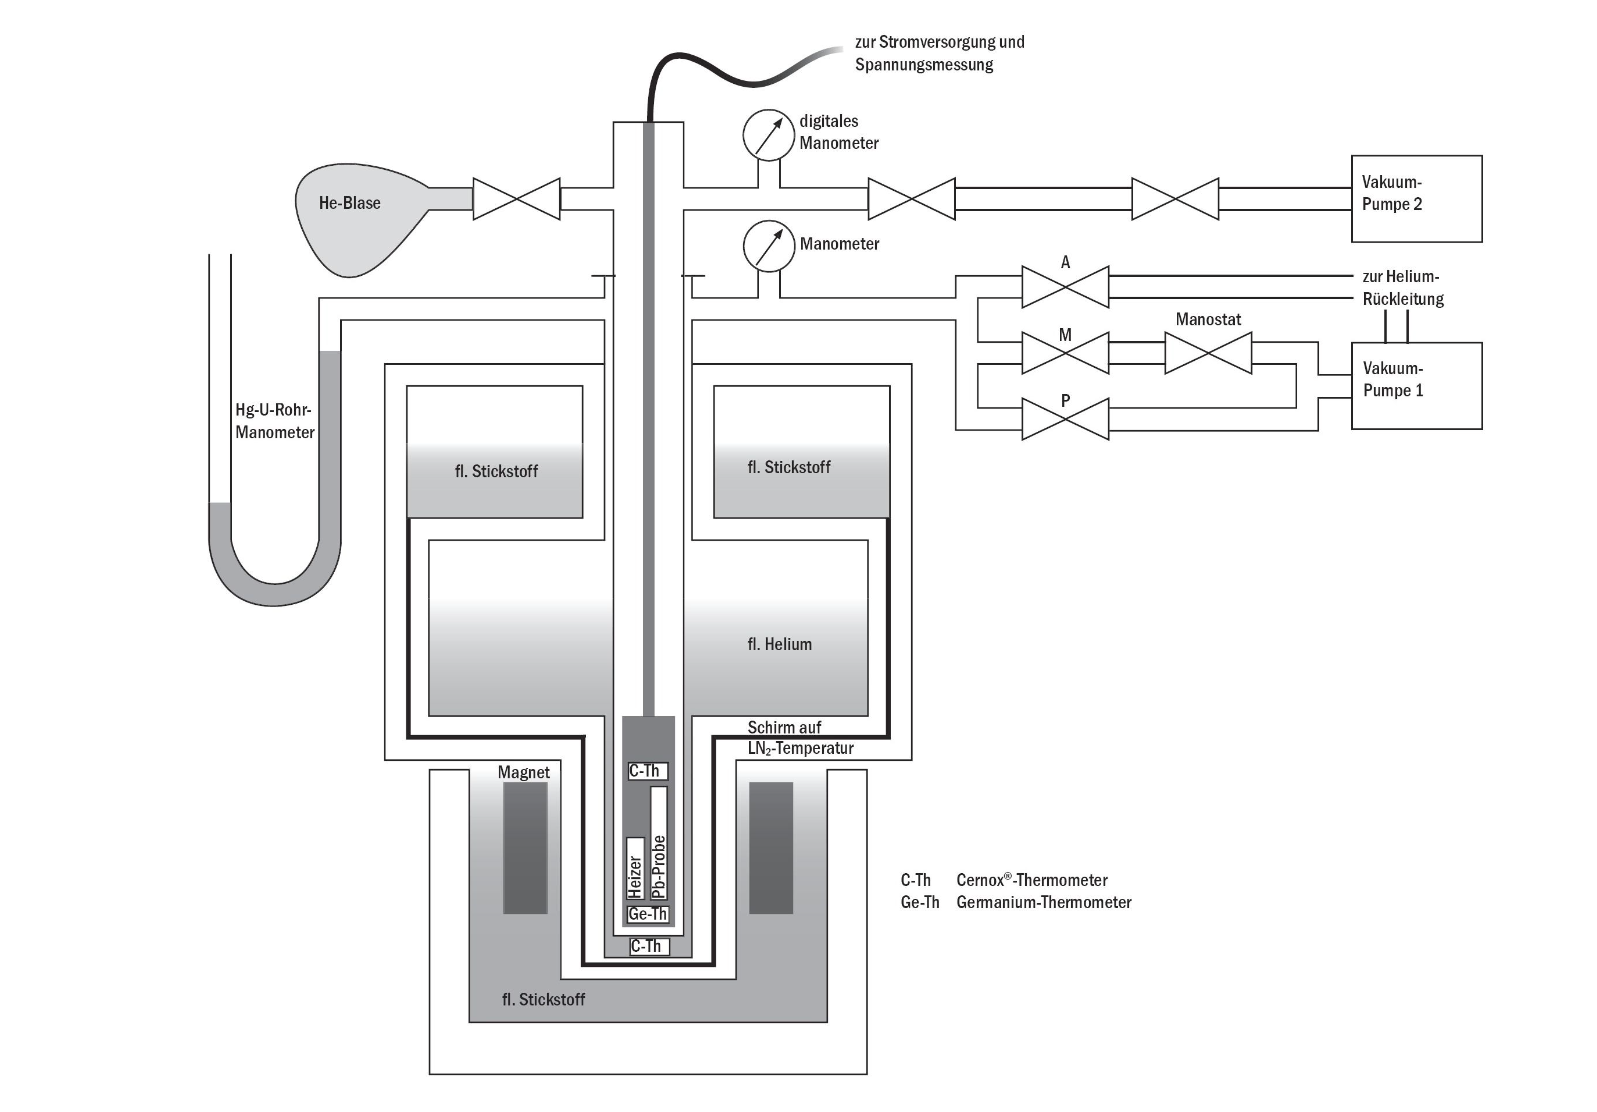
\includegraphics[width=0.8\linewidth]{su2_aufbau.png}
    \caption{Aufbau des Badkryostaten, der in diesem Versuch benutzt wird \cite{Platzanleitung}.}
    \label{fig:aufbau}
\end{figure}
Um die kritische Temperatur von Blei $T_c= \SI{7.2}{\kelvin}$ zu erreichen, wird ein Badkryostat benutzt.\\

\section{Aufbau und benutzte Geräte}
    \begin{itemize}
        \item Badkryostat (LHe, LN2), Fa. CryoVac 
        \item Helium-Levelmeter HLG200, Fa. Cryogenics 
        \item Temperature-Controller LS340, Fa. Lake Shore: Sensor A: Cernox - Thermometer am Boden des Kryostats, Sensor B: Cernox - Thermometer auf dem Probenhalter 
        \item Stromquelle für Magnet CONRAD PS2403 D 
        \item Stromquelle für Probe Statron Typ 3207 
        \item Stromquelle  für  Germanium-Thermometer  (auf  dem  Probenhalter)  LS120,  Fa. Lake Shore 
        \item DC-Digitalvoltmeter Keithley 2700 (mit 10-Kanal-Einschub, relaisgeschaltet) 
        \item Drehschieberpumpe MLW 4 m3/h (Pumpe 2) zur Evakuierung des Probenraums 
        \item Drehschieberpumpe mit Manostat (Pumpe 1) zum Abpumpen über dem Heliumbad 
        \item Computer, inkl. IEEE-Inteface 
    \end{itemize}

\section{Versuchsdurchführung}\label{Durchfuhrung}
Zuerst wurde der Badkryostat mit $\ce{LN2}$ in den äußeren Kammern auf etwa 140K abgekühlt, um weniger LHe verbrauchen zu müssen. Dann wurde der Kryostat mit LHe auf $T=4.2 \si{K}$ abgekühlt und ein Bild vom Gasmengenzähler zur späteren Bestimmung des He-Verbrauchs gemacht. Der Zähler zeigte zu Beginn $\SI{409.024}{m^3}$ an. Schließlich wurde auch die Spule mit $\ce{LN2}$ gekühlt, um die nötigen Feldstärken ohne Überhitzen zu generieren. \\
\subsection{Vorversuch: Einfluss von Probenstrom und Stromrichtung}
Zuerst wurde der Einfluss des Probenstroms auf das notwendige kritische Feld ermittelt. Dazu wurden fünf Messungen bei 4.2\,K aufgenommen, bei den Stromstärken $I_\mathrm{Probe}\in\{\SI{0.18}{A},\SI{0.29}{A},\SI{0.09}{A},\SI{-0.9}{A},\SI{-0.20}{A} \}$. Die negativen Stromstärken kommen durch Umpolung zustande. Die Messergebnisse als Diagram sind in \bcref{fig:pretrial} dargestellt.
\subsection{Abkühlmodus}
Alle folgenden Versuche wurden bei \SI{0.18}{A} Probenstrom durchgeführt.\\
Mittels Abpumpen des Heliumdampfes kann eine weitere Abkühlung des Kryostaten erreicht werden. Dazu wird mittels eines Manostaten der Druck konstant gehalten, um eine Messung unter konstanten Bedingungen zu ermöglichen. Dies erlaubt es, Temperaturen bis etwa 2\,K zu erreichen. Wenn der Manostat entfernt wird, kann durch die vorhandene Vakuumpumpe eine Temperatur von 1.77\, K erreicht werden.\\ Zu jeder gemessenen Temperatur wird durch das Messprogram der Druck über dem Gas, die Temperatur eines Cervex-Thermometers und die Spannungen an einem Germanium-Thermometer, an der Spule, am Bleidraht, sowie über einen Widerstand mit dem Bleidraht in Reihe geschalten, gemessen. \\Die Spannungen können durch in Reihe geschaltete Widerstände ($\SI{1}{\Omega}$ für den Spulenstrom, $\SI{10}{\Omega}$ für den Probenstrom) in Ströme umgerechnet werden. \\Die Abhängigkeit $R_\mathrm{Blei}(H)$ ist im Anhang in \cref{fig:RH} für alle Temperaturen dargestellt, zu den Temperaturen siehe \bcref{Temperatures}.
\subsection{Heizmodus}
Statt dem Gas über dem LHe wird jetzt das Transmissionsgas (auch He) abgepumpt, um die Probe ein Stück weit zu isolieren und die Heizung somit effizienter zu machen. Nun wird an dem Controller der elektrischen Heizung ein Soll-Temperaturwert eingegeben, die dann selbständig angesteuert wird.\\
Da die letzten 0.05\,K Differenz sehr langsam überbrückt werden, wird mit der%TODO verschweigen wir das lieber? JA
Messung schon ab dort begonnen. Im Heizmodus ist der Dampfdruck nicht mehr aussagekräftig (weil er nicht mehr zur Temperaturregulierung benutzt wird) und wird deswegen in der Auswertung nicht mehr benutzt. Alle andere Auswertung ist an den gleichen stellen zu finden. \\
Am Ende des Experiments (etwas verspätet, da der Betreuer nicht gefunden wurde) wird noch einmal die Anzeige des Gasmengenzählers abgelesen, die zu diesem Zeitpunkt $\SI{416.185}{m^3}$ anzeigt.
\section{Auswertung}
\paragraph{Magnetfeld}
Das Magnetfeld wird von einer Zylinderspule erzeugt, in derem Inneren die Probe sitzt. Die Spule kann näherungsweise als lange Spule
betrachtet werden, die Permeabilität $\mu_r$ wird, da die Probe sich in dünnem Gas befindet als $\approx1$ abgeschätzt, wodurch sich das

Magnetfeld wie folgt ergibt:
\[
H = \frac{N}{l}\cdot I = \SI{23400}{I/m}.
\]

\subsection{Vorversuch}
Im Vorversuch wurde bei der selben Temperatur (4.2K) fünf verschiedene Stromstärken durch die Probe gesendet, um den Einfluss dieser Stromstärken auf die Messung abzuschätzen. Die Diagramme in \bcref{fig:pretrial} wurden dabei aufgenommen.
\begin{figure}
    \centering
    \caption{Messkurven der Vorversuche}
    \includesvg[height=1.1\textheight]{pretrial.svg}
    \label{fig:pretrial}
\end{figure}
Aus diesen wurde mit der in \bcref{Hc} beschriebenen Methode das kritische Feld ausgelesen und in \bcref{fig:Hcpretrial} eingezeichnet. Die Unsicherheit unserer Messung wird damit auf 3500/2 \si{\frac{A}{m}} abgeschätzt. Die erwartete Symmetrie um 0 ist gegeben, auch wenn das Feld für umgepolte Spannung schneller abfällt als im ursprünglichen Modus. Für eine Diskussion der Hintergründe siehe \bcref{diskussion}
\subsection{Bestimmung des Kritischen Feldes}\label{Hc}
Um das kritische Feld $H_c$ mittels des \say{Midpoint}-Kriteriums automatisiert zu bestimmen, muss zuerst der Übergangsbereich bestimmt werden. Dazu wird mittels \verb+curve_fit+ für jeden Messpunkt über eine bestimmte $H$-Distanz im $H-R$ Diagramm voraus (in diesem Fall $0.2\cdot23400\,\si{\frac{A}{m}}$ , der zweite Faktor ist der Umrechnungsfaktor von Spulenstrom zur Flussdichte) 
die mittlere Steigung der Messpunkte ermittelt. Übersteigt diese einen kritischen Wert (in diesem Fall $\SI{1/23400}{\frac{m\Omega}{Am^{-1}}}$), wird die Überprüfung abgebrochen und der Messpunkt wird zum Beginn der Übergangszone deklariert. Die Messreihe bis dorthin wird linear gefittet, der y-Wert des Fits am Übergangsort wird zu 0\% (bzw. 100\%) der Übergangshöhe. Mit diesen Werten werden dann H-Werte für 10\%, 90\% und 50\% der Sprunghöhe ermittelt. Alle Plots der Einzelmessungen, genau wie die interessanten Skriptausschnitte sind im Anhang zu finden. Man erhält die kritischen Feldstärken in \bcref{tab:Hclist}.

\begin{figure}[!htp]
    \centering
    \includesvg[width=0.705\linewidth]{HcPlot.svg}
    \caption{Phasenlinie zwischen normalleitendem und supraleidendem Zustand. Der Abszissenabschnitt entspricht der kritischen Temperatur, der Ordinatenabschnitt $H_{c0}$.}
    \label{fig:Hcplot}
\end{figure}
\pagebreak
\begin{wraptable}{r}{5cm}
    \centering
        \caption{Kritische Felder in Abhängigkeit von der Temperatur}
    \begin{tabular}{c|c}
        T/K & $H_c$/\si{\frac{A}{m}}  \\\hline \hline
 1.77&61401.14\\
2.13&59273.97\\
2.20&58398.42\\
2.39&57052.58\\
2.59&55285.81\\
2.90&51909.80\\
3.16&49325.30\\
3.46&46211.14\\
3.76&43245.18\\
4.02&40150.86\\
4.23&38222.56\\
4.50&35637.10\\
4.80&31800.29\\
5.10&28016.53\\
5.40&23211.25\\
5.70&18039.26\\
6.00&13646.44\\
6.30&8201.40\\
6.60&3154.26\\
    \end{tabular}
    \label{tab:Hclist}
\end{wraptable}
Mit den Werten aus \bcref{tab:Hclist} wurde \bcref{fig:Hcplot} erstellt. Man passt an die Messdaten den erwarteten Zusammenhang
\[
H_c(T)=H_{c0}(T)\cdot\left(1-\left(\frac{T}{T_c}\right)^2\right)\label{eq:Hc}
\]
an, mit den Fitparametern $H_{c0}$ und $T_c$. Es ergibt sich:
\[
H_{c0}= \SI{6.45194388e+04}{\frac{A}{m}},\: T_c = \SI{6.73060460}{K}
\]
Um die Unsicherheit dieser Werte abzuschätzen wird $\dfrac{H_{c, \mathrm{max}}-H_{c, \mathrm{min}}}{2}=1750\,\si{\frac{A}{m}}$ aus dem Vorversuch als Fehler genutzt und die minimal und maximal so möglichen Verläufe von \bcref{eq:Hc} eingezeichnet. Die halbe Differenz ihrer Fitparameter gibt dann die Unsicherheit der oben bestimmten Werte:
\[
\Delta H_{c0}= \SI{0.18e+04}{\ampere \per \meter},\: \Delta T_c = \SI{0.09}{K}.
\]
In \cite{TN_libero_mab2} wird für die kritische Flussdichte ein Wert von 
$
H_{c0}=802.6\pm0.4\,\si{G}
$
angegeben, was in unsere Feldstärke mit dem Faktor $\frac{1}{10000\mu_0}$ umgerechnet werden kann. Dies ergibt:
\[
H_{c0}=63870\pm32\,\si{G}
\]

\begin{figure}[htp!]
    \centering
    \includesvg[width=0.63\linewidth]{h8_699.svg}
    \caption{Messung bei $6.99\,$K. Das Minimum des Widerstandes liegt weit oberhalb des in der Supraleitenden Phase erwarteten.}
    \label{fig:overcrit}
\end{figure}
Die Differenz zwischen den Werten beträgt $\SI{0.065e4}{{\frac{A}{m}}}$, weit weniger als unsere Messunsicherheit. \\Allerdings gibt \cite{Pearson} für $T_c=7.175\,$K an, deutlich mehr als in unserem Experiment. Unser Wert wird aber auch durch eine Messung bei 6.9K untermauert (s. \bcref{fig:overcrit}), bei der das Midpoint-Kriterium schon kein $H_c$ mehr liefern würde.

\subsection{Bestimmung der Übergangsbreiten}
Man erkennt in \bcref{fig:uebergang}, dass die Übergangsbreite für niedrige Temperaturen konstant ist und dann ab $4\,$K etwa linear abfällt. Diese Abnahme fällt mir der Aufnahme des Heizmodus zusammen, aber auch mit geringeren Werten für $H_c$. Die Erklärung könnte also einerseits in dem geänderten Experimentellen Umständen zu finden sein (etwa erhöht sich die Temperatur im Heizmodus auch nach Beginn der Messreihe noch durch die Natur des Temperaturcontrollers etwas, was die Übergangsbreite schmälern würde) oder darin, dass das Material empfindlicher auf das Feld reagiert, wodurch sowohl $H_c$ als auch $\Delta_H$ bei höheren Temperaturen schmäler würden.
\begin{figure}
    \centering
    \includesvg[width=1.1\linewidth]{uebergang.svg}
    \caption{Die Übergangsbreite $\Delta_h$. Man erkennt eine Fluktuation um \SI{12000}{\ampere\per\meter} bei niedrigen Temperaturen, dann einen linearen Abfall hin zu den höheren Temperaturen.}
    \label{fig:uebergang}
\end{figure}

\subsection{Überprüfung der Kalibrierung des Ge-Thermometers}\label{Temperatures}
Es ist bekannt, dass der elektrische Widerstand in einem Halbleiter mit der allgemeinen Beziehung:
\begin{equation}
    R \propto \exp(-\alpha \cdot T)
\end{equation}
beschreibbar ist. Man setze für den Gesamtausdruck an:
\begin{equation}
    R(T) = A\cdot \exp(-B\cdot T)
\end{equation}
woraus sich für den gesuchten Ausdruck für die Temperaturabhängigkeit ergibt:
\begin{equation}
    T(R) = -\frac{1}{B}\cdot \ln{\frac{R}{A}}
    \label{eq:T(R)}
\end{equation}

Mittels \verb+scipy.optimize.curve_fit+ werden die $(R,T)$-Datenpunkte an \bcref{eq:T(R)} gefittet.\\
Man erhält folgende Parameter samt der durch die Kovarianz-Matrix ermittelten, als statistisch interpretierten Messunsicherheiten:
\begin{align*}
A\pm\Delta A&=(27471\pm998)\,\si{\ohm}\\
B\pm\Delta B&=(766\pm11.3)\cdot 10^{-3}\,\si{\per\kelvin}
\end{align*}
\begin{figure}[h!]
    \centering
    \includesvg[width=1.1\linewidth]{Ge_T(R)FINAL.svg}
    \caption{Fit der Messdaten an die Fitfunktion $T(R)=-\frac{1}{B}\cdot \ln{\frac{R}{A}}$ aufgrund der bekannten Relation. Auf das Einzeichnen der Fehlerbalken wurde aufgrund der Nichtsichtbarkeit dieser (relative Messunsicherheit für alle Messpunkte im Bereich $\frac{\Delta T_i}{T_i}\approx \num{e-5}$).}
    \label{fig:T(R)}
\end{figure}
Man sieht für den Messpunkt bei ca. $R=8300\si{\ohm}$ eine relative große Abweichung von der Fitkurve. \\
Dies ist wahrscheinlich darauf zurückzuführen, dass das Germanium-Thermometer nur für Temperaturen bis $T\ge\SI{1.5}{\kelvin}$ ausgelegt ist und deshalb Ungenauigkeiten in diesem Grenzberereich auftreten können.\\
Untermauert wird diese Annahme dadurch, dass durch Vergleich mit der\\ $^{4}$He-Dampfdrucktabelle aus \cite{Platzanleitung} klar wird, dass für den gemessenen Druck zu diesem Widerstand ($p_{Mess.}=\SI{7}{\mmHg}$) für einen sehr naheliegenden in der Tabelle \\($p_{Tabelle} = \SI{7,0476}{\mmHg}$) die Temperatur $T_{Tabelle}=\SI{1.65}{\kelvin}$ statt der gemessenen 
$T_{Mess.}=\SI{1.77}{\kelvin}$ relativ stark abweicht.\\\\
Neben der Dampfdrucktabelle gibt es als Referenz auch noch eine alte Eichtabelle des Ge-Thermometers, welche ebenfalls in \cite{Platzanleitung} zu finden ist.\\
Im Folgenden werden die verschiedenen Temperaturmessmöglichkeiten verglichen.\\\\
Die Messmethode über den Widerstand wurde mit der Fitfunktion $T(R)$ beschrieben. Diese soll nun mit den anderen beiden Messmöglichkeiten: $  ^{4}$He-Dampfdrucktabelle und alte Ge-Eichtabelle verglichen werden.\\
Hierzu werden die Differenzen $T(R)-T(p)$ bzw. $T(R)-T_{Eich}(R)$ gegen $T(p)$ bzw. $T_{Eich}(R)$ aufgetragen.\\
Da die verschiedenen Funktionen von Druck bzw. elektrischem Widerstand abhängen, wird so vorgegangen: Für $T(R)-T(p)$ werden für $T(p)$ die gemessenen Drücke mit denen der Dampfdrucktabelle abgeglichen (bis $\SI{4.2}{\kelvin}$), wobei die gemessenen Drücke freilich nicht genau mit denen der Tabelle übereinstimmen, wird der nächstgelegene Druck aus der Tabelle für die jeweilige Messung benutzt, wobei \bcref{tab:pvsp} die Wahl dieser Methode rechtfertigt. Die zu den gemessenen Drücken, die verwendet werden zugehörigen Widerstände, werden in $T(R)$ eingesetzt und die Differenz der jeweils zugehörigen Temperaturen in \bcref{fig:tvst12} geplottet.\\
\begin{table}[!h]
    \centering
    \caption{Relative Abweichung der gemessenen Drücke, von denen aus der Dampfdrucktabelle}
    \begin{tabular}{c|c|c}
    $p_{Tab.} / \si{\mmHg}$& $p_{Mess} / \si{\mmHg}$&$ \frac{p_{Tab.} - p_{Mess}}{p_{Tab.}}$\\ \hline \hline
    7.048 & 7 & 0.00(7) \\
    35.88 & 35.85 & 0 \\
    40.58 & 41.049 & -0.01   \\
    63.48 & 63.45 & 0 \\
    93.99 & 99.97 & -0.06  \\
    175.57 & 183.29 & -0.04 \\
    277.63 & 277.13 & 0.00(2) \\
    425.28 & 417.01 & 0.02 \\
    587.63 & 601.85 & -0.02 \\
    787.43 & 801.86 & -0.02
    \end{tabular}
    \label{tab:pvsp}
\end{table}
Es sei hier noch erwähnt, dass anfangs versucht wurde anhand der Wertepaare der Dampfdrucktabelle eine Fitfunktion für $T(p)$ zu finden, wobei diese in Form von\\ $T(p)=\sqrt{A\cdot p} + B$ anfangs als aussichtsreiche Kandidatin erschien, was jedoch verworfen wurde.\\\\
Nun sollen die bisherigen Kalibrierungspunkte der Ge-Eichtabelle überprüft werden. Hierzu werden die Eichwiderstände in die Fitfunktion eingesetzt und wieder die Differenz gebildet und über den Eichtemperaturen geplottet (auch zu sehen in \bcref{fig:tvst12}).\\
\begin{figure}[!htp]
    \centering
    \includesvg[width=1.1\linewidth]{TvsT12relohnebetrag.svg}
    \caption{Relative Abweichungen der verschiedenen Temperaturen $T_{fit}(R)$, $T(p)$ und $T(R)_{Eich}$.}
    \label{fig:tvst12}
\end{figure}

\subsection{Bestimmung der Länge des Drahtes}
Als Zusatzaufgabe soll die Länge des Bleidrahtes aus den gemessenen Widerstandswerten abgeschätzt werden.\\
Hierzu bedient man sich des Ausdrucks für den spezifischen Widerstand $\rho$ (wobei $l$ die Länge des Drahtes, $R$ der gemessene Widerstand und $A = \pi r^2$ die Fläche des als zylinderförmig approximierten Drahts mit Radius $r$ ist):
\begin{equation}
    R = \frac{\rho\cdot A}{l} \Longleftrightarrow l = \frac{R\cdot \pi r^2}{\rho}
\end{equation}
Für den spezifischen Widerstand wird folgende linearisierte Formel verwendet, wobei $T_0 = \SI{293.15}{\kelvin}$ die Bezugstemperatur ist:
\begin{equation}
    \rho(T) = \rho(T_0)\cdot (1+\alpha\cdot(T-T_0))
\end{equation}
Hierbei ist $\alpha$ der Temperaturkoeffizient und $\rho(T_0)$ ein Eichwert bei bekannter Temperatur der einer Tabelle entnommen wird.\\
$\alpha$ ist selbst auch temperaturabhängig, jedoch gibt es einen Eichwert bei $T=\SI{20}{\celsius}$, der herangezogen wird.\\
Der Draht hatte in dem gemessenen Zeitraum die Durchschnittstemperatur $T=\SI{291.801}{\kelvin}$. \\
R lässt sich zu $\SI{3.6}{\ohm}$ bestimmen (Mittelwert über $N=12$ Messpunkte).\\\\
Bekannte Werte sind: $ \rho(T_0) = \SI{0.208}{\ohm \mm\squared\per \meter}$ und $\alpha(T_0) = \SI{4.2 e-3}{\per \kelvin}$\cite[14-1]{smithells}.
\\Somit ergibt sich insgesamt für die Länge in Abschätzung (da die tatsächliche Temperatur $T$ leicht von $T_0$ abweicht):
\begin{equation}
    l_{Draht} = \SI{0.86}{\meter}
\end{equation}

\subsection{LHe-Verbrauch}
Die Differenz zwischen den Zählerständen beträgt (siehe \bcref{Durchfuhrung}):
\[
\mathrm{GHe-Verbrauch}=(416.185-409.024)\,\si{m^3}=7.161\,\si{m^3}
\]
Aus der Anleitung entnimmt man als Umrechnungsfaktor 700\,l GHe $\cong$ 1\,l FHe. Damit folgt, dass 10.23\,l LHe verbraucht wurden.
\subsection{Ergebnisse}
\begin{align*}
    H_{c0}&=\SI{6.45\pm0.18e4}{\ampere\per\meter}\\
    T_c&=\SI{7.73\pm0.09}{K}\\
    l_{Draht}&= \SI{0.86}{\meter}
\end{align*}

\section{Diskussion}\label{diskussion}
Die im Vorversuch beobachtete Variation des kritischen Feldes kann wahrscheinlich auf durch den Strom im Leiter erzeugte Felder zurückgeführt werden, die zusätzlich zum externen Feld beitragen.\\
Die ermittelte kritische Feldstärke bei 0\,K von $H_{c0}=\SI{6.45e4}{\ampere\per\meter}$ eingerechnet seiner Fehler liegt ausreichend nah beim Literaturwert von $\SI{6.389e4}{\ampere\per\meter}$. Allerdings weicht der Wert der kritischen Temperatur deutlich vom Literaturwert von 7.2\, K ab, weit mehr als innerhalb der Fehler der Messung möglich ist. Dies schließt auch systematische Fehler der Temperaturmessung ein, die vom Hersteller mit 4\,mK angegeben werden\cite{Cernox}. Zusätzlich weißt auch unsere Messung bei 7\,K kein kritisches Feld nach dem Midpoint-Kriterium auf, was hier als Abwesenheit eines supraleitenden Zustandes interpretiert wird. Allerdings ist noch ein für Supraleitung typischer Abfall des Widerstandes bei sehr schwachen Magnetfeldern zu beobachten, nicht mehr jedoch auf den vorher üblichen sehr niedrigen Widerstand. Die Abweichung könnte daher stammen, dass in der Literaturangabe auch dieser schwache Abfall noch als Supraleitend gewertet wird.
\footnote{Tatsächlich passt das kritische Feld, wenn nicht nach dem Midpoint-Kriterium, sondern ab 90\% der Übergangshöhe ermittelt, deutlich besser auf die quadratische Funktion an die es gefittet wurde, wie in \bcref{fig:Hc90} im Anhang erkennbar ist. Dies ändert freilich wenig an der falschen kritischen Temperatur ändert.}\\\\
Die negativen Widerstände (verursacht durch eine negative Spannungsmessung) in der supraleitenden Phase können von den Experimentatoren nicht theoretisch erklärt werden, weshalb wir die Gründe für diese im Versuchsaufbau suchen müssen. Allerdings sind die systematischen Fehler der Spannungsmessung nicht groß genug um diese zu erklären. Auffällig ist, dass der Effekt bei schwachen Strömen durch die Probe stärker auftritt als bei starken strömen, und bei den Messungen mit umgepoltem Strom gar nicht. Es wäre also angezeigt gewesen, die Messungen mit umgepoltem Probenstrom durchzuführen.\\\\
Die \say{alte} Kalibrierung des Ge-Thermometers weißt relativ große Abweichungen zu den gemessenen Temperaturen in den Bereichen $T \le \SI{2.5}{\kelvin}$ bzw. $T \ge  \SI{4}{\kelvin}$ auf.\\
Eine Verbesserung Kalibrierung des Cernox-Ge-Thermometers könnte man gewährleisten in dem man die nun gemessenen Werte weiterhin als Referenz nutzt (bestenfalls eine neue Messung tätigt mit so vielen Messpunkten, wie möglich).\\
Weiterhin scheint eine Ausbesserung der Eichtabelle vor allem dort sinnvoll, wo sowohl die Differenz mit der $T(p)$, als auch mit $T_{Eich}(R)$ das gleiche Vorzeichen hat, ergo im Bereich $\SI{2.0}{\kelvin} \le T \le \SI{3.5}{\kelvin}$.\\
Außerdem konnte die Länge des Bleidrahtes auf einen Wert $l \approx \SI{0.9}{\meter}$ bestimmt werden, der dem Referenzwert $l \approx \SI{1}{\meter}$ sehr nahe kommt.
\setcounter{biburllcpenalty}{7000}
\setcounter{biburlucpenalty}{8000}
\printbibliography
\pagebreak
\section{Anhang}
\subsection{Messergebnisse}
\begin{table}[!htp]
    \centering
    \begin{tabular}{c|c|c|c}
         $\bar{\si{T}}/\si{\kelvin}$&$\bar{\si{p}}/\si{mmHg} $&$U_{Ge}/\si{\volt}$&$R_{Ge}/\si{\ohm}$\\ \hline \hline
         1.773  & 7       & 0.828  & 8283   \\
        2.127  & 35.85   & 0.519  & 5194   \\
        2.202  & 41.05   & 0.488  & 4883   \\
        2.391  & 63.45   & 0.422  & 4222   \\
        2.585  & 99.97   & 0.361  & 3608   \\
        2.903  & 183.26  & 0.282  & 2819   \\
        3.161  & 277.13  & 0.232  & 2322   \\
        3.457  & 417.01  & 0.189  & 1886   \\
        3.76   & 601.85  & 0.154  & 1544   \\
        4.025  & 801.86  & 0.131  & 1310   \\
        4.232  & 976.52  & 0.116  & 1161   \\
        4.503  & 985.87  & 0.101  & 1011   \\
        4.805  & 986.31  & 0.078  & 792    \\
        5.098  & 987.59  & 0.06   & 601    \\
        5.397  & 987.35  & 0.045  & 453    \\
        5.696  & 988.02  & 0.035  & 347    \\
        6      & 986.97  & 0.026  & 263    \\
        6.299  & 986.14  & 0.02   & 201    \\
        6.597  & 987     & 0.016  & 160   
    \end{tabular}
    \caption{Die jeweiligen Werte sind Mittelwerte, der bei der Variation des Spulenstroms von 0 bis 3A aufgenommenen Werte (im Durchschnitt 30-40). Die Messunsicherheiten berechneten sich als Standardabweichungen des Mittelwerts zu relativen Messunsicherheiten, die bei keiner der Größen $p, T, U_{Ge}, R_{Ge}$ größer, als $\num{e-3}$ wurden. Deshalb wurde darauf verzichtet diese hier noch einmal explizit darzustellen.}
    \label{tab:my_label}
\end{table}
\pagebreak
\subsection{Graphen der Einzelmessungen}
\begin{figure}[!htp]
    \centering
    \includesvg[height=0.85\textheight]{simples1.svg}
    \caption{Einzelmessung mit gekennzeichneten Übergangszonen und kritischen Feldern}
    \label{fig:RH}
\end{figure}
\begin{figure}[!htp]
    \centering
    \includesvg[height=0.85\textheight]{simples2.svg}
\end{figure}
\begin{figure}[!htp]
    \centering
    \includesvg[height=0.4\textheight]{simples3.svg}
\end{figure}
\begin{figure}
    \centering
    \includesvg[height=0.5\textheight]{HcPretrial.svg}
    \caption{$H_c$ in Abhängigkeit von I. Die erwartete Symmetrie um $I=0$ ist hinreichend gegeben, auch wenn die umgepolte Messung schneller abfällt.}
    \label{fig:Hcpretrial}
\end{figure}
\begin{figure}
    \centering
    \includesvg[height=0.6\textheight]{HcPlot90.svg}
    \caption{Kritische Feldkurve wenn $H_c$ bei 90\% der Sprunghöhe angesetzt wird. Besserer Fit im Vergleich mit \bcref{fig:Hcplot}, v.a. im Niedertemperaturbereich.}
    \label{fig:Hc90}
\end{figure}
\clearpage
\subsection{Skripts}
\paragraph{Bestimmung des Übergangspunktes}
\begin{verbatim}
    def local_lin(x, y):
    """
    Testet bis wohin das Eingabearray lokal weniger als vorgegeben steigt

    Parameters
    ----------
    x, y: Arrays

    Returns
    -------
    i : letzter Index an dem y(x) flach genug ist

    """
    
    slope = 0
    lim = 0.0001*10000*23400
    i = 0
    j = 0
    dx = 0.2*23400
    while abs(slope) < lim:
        j = 0 # Bestimmt den Index, ab dem die vorgegebene x-Länge erreicht ist
        while abs(x[i+j]-x[i]) < dx:
            j += 1
        if j<3:  # Falls die Messwerte sehr weit auseinander liegen
            j = 3
        
        x_loc = x[i:i+j]
        y_loc = y[i:i+j]
        popt, pcov = curve_fit(linear, x_loc, y_loc)
        i += 1
        slope = popt[0]
        
    if i<2:     # Falls der flache Bereich sehr kurz ist
        i = i + int(j/3)
    return i
\end{verbatim}
\paragraph{Bestimmung der relevanten Übergänge}
\begin{verbatim}
    # Vorverarbeitung der Daten
    H_sort = np.sort(I_coil)
    R_sort = V_sample[np.argsort(I_coil)]/V_sample_i[np.argsort(I_coil)]*1000
    # Bestimmung der Übergangsgrenzen
    lim_low = local_lin(H_sort, R_sort)
    lim_up = local_lin(H_sort[::-1], R_sort[::-1])
    lim_up = len(p) - lim_up
    
    paramsl, pcov = curve_fit(linear, H_sort[0:lim_low], R_sort[0:lim_low])
    paramsu, pcov = curve_fit(linear, H_sort[lim_up:], R_sort[lim_up:])
    
    # Bestimmung der Grenzen des Übergangs
    R_low, R_high = linear(H_sort[lim_low], *paramsl), linear(H_sort[lim_up], 
                                                              *paramsu)
    R_mod = R_sort - R_low
    R_height = R_high - R_low
    R_crit = R_height*0.5 + R_low
    # Finde nächsten Messpunkt an gewünschtem Widerstand
    i_start = (np.abs(R_mod - R_height*0.1)).argmin()
    i_end = (np.abs(R_mod - R_height*0.9)).argmin()
    
    # Bestimmung des Kritischen Feldes
    paramss, pcov =  curve_fit(linear, H_sort[i_start:i_end], 
    R_sort[i_start:i_end])
    H_c = (R_crit - paramss[1])/paramss[0]
    transition[i] = [H_c, abs(H_sort[i_end] - H_sort[i_start])]
\end{verbatim}
\end{document}